% Need to fix optimization problems -- add spacing between min and obj
%#######################################################################

In the previous chapter, we showed how local search heuristics produced
parcels that were balanced and had high within-parcel and low
between-parcel edge weights. The central idea behind such methods
was to choose vertices to be in the same component if the edge
connecting them has high distance correlation. Vertices were added to
components one-by-one with constraints on component size, but not on
component shape. As a result, one salient issue with these
parcellations was lack of smoothness, or regularity in the parcels'
spatial shapes. There was scant resemblence between the anatomical maps
of the brain depicting smooth, rotund lobes and our jagged, web-like
parcellations.

One key reason for this phenomenon are the local search heuristics'
focus on maximizing \textit{average} within-component edge weights
(equivalently, minimizing \textit{average} between-component edge
weights because edges are either within the same component or between
different components). To get smoothness in the boundary between
components, we could either impose a penalty for too many
between-component edges and work that into the local search heuristics,
or try minimizing over the sum of all weights on between-component
edges. This chapter deals with the second approach and this family of
methods is called spectral partitioning.

Spectral partitioning constitutes the second major class of techniques
used to partition graphs. Rather than rely on local component-growing
heuristics, spectral partitioning uses information about the entire
graph at once.

Throughout this chapter, a valid partitioning
$P_k = (V_1, ..., V_k)$ of the graph $G = (V, E)$ is defined in the
same way as in chapter 3; i.e., it must satisfy

\begin{enumerate}[1.]
\item
$V_i \neq \emptyset$ for all $V_i \in \mathcal{P}_k$

\item
$\bigcup\limits_{i=1}^k V_i = V$

\item
$V_i \cap V_j = \emptyset$ for all $V_i, V_j \in \mathcal{P}_k$

\item
$V_i$ is connected (i.e. for every two vertices in $V_i$, there is a
path between them) for all $V_i \in \mathcal{P}_k$
\end{enumerate}

For all edges $(i,j) \in E$, let $w_{ij}$ denote the weight of the edge
connecting vertices $i$ and $j$.
$S^{n \times n}$ is the set of real symmetric $n \times n$ matrices.
We further define, for a given graph $G = (V, E)$, the associated

\begin{definition}
Adjacency matrix. $A \in \mathcal{S}^{n \times n}$ has entries
\[
A_{ij} = \begin{cases}
  w_{ij} & \text{if } (i,j) \in E \\
  0      & \text{otherwise} \\
\end{cases}
\]
\end{definition}

\begin{definition}
Degree matrix. $D \in \mathcal{S}^{n \times n}$
\[
D_{ij} = \begin{cases}
  \sum_{k = 1}^n A_{ik} & \text{if } i = j \\
  0                     & \text{otherwise} \\
\end{cases}
\]
\end{definition}

\section{Size-Constrained MinCut and Graph Bipartitioning}

Consider the case $k = 2$. For all $i \in V$, let $x_i = 1$ if
$i \in V_1$ and $x_1 = -1$ if $i \in V_2$. Then the sum of weights on
edges between the two components is
\begin{align*}
C(P_2)
&= \sum_{i \in V_1} \sum_{j \in V_2} A_{ij} \\
&= \sum_{i = 2}^n \sum_{j = 1}^{i-1} \frac{(x_i - x_j)^2}{4} A_{ij} 
\end{align*}
since
\[ (x_i - x_j)^2 = \begin{cases}
	4 & \mbox{if } i,j \mbox{ are in different components} \\
	0 & \mbox{otherwise}
\end{cases}\]

$C(P_2)$ can also be written in a matrix quadratic form, as

\begin{align*}
C(P_2)
&= \sum_{i = 2}^n \sum_{j = 1}^{i-1} \frac{(x_i - x_j)^2}{4} A_{ij} \\
&= \frac{1}{2} \sum_{i,j = 1}^n \frac{(x_i - x_j)^2}{4} A_{ij} \\
&= \frac{1}{2} \sum_{i,j = 1}^n
   \frac{x_i^2 + x_j^2 - 2 x_i x_j}{4} A_{ij} \\
&= \frac{1}{2} \sum_{i,j = 1}^n \frac{1 - x_i x_j}{2} A_{ij} \\
&= \frac{1}{4} \sum_{i,j = 1}^n (x_i^2 - x_i x_j) A_{ij} \\
&= \frac{1}{4} \sum_{i = 1}^n x_i^2 \sum_{j = 1}^n A_{ij}
 - \frac{1}{4} \sum_{i,j = 1}^n x_i A_{ij} x_j \\
&= \frac{1}{4} \sum_{i = 1}^n x_i^2 D_{ii} - \frac{1}{4} x^T A x \\
&= \frac{1}{4} x^T (D - A) x \\
&= \frac{1}{4} x^T L x
\end{align*}
where $L$ is called the Laplacian matrix of the graph and defined as
$L = D - A$. MinCut can thus be formulated as minimizing $x^T L x$
subject to $x \in \{-1, 1\}^n$.

Algorithms like Karger's can solve MinCut in polynomial time. However,
MinCut in this formulation lacks constraints on the size of the
partitions, and if applied to our brain parcellation problem, would
result in severely inbalanced partitions. If constraints on the sizes
of the components were added, the problem becomes NP-hard [citation].

An old but effective approach to bipartitioning uses the eigenvectors
of the Laplacian matrix and is called spectral bipartitioning.
The approach relaxes the $\{-1, 1\}$ constraint on $x$ (and rescales
$x$) so that it need only satisfy $\|x\| = 1$ ($\|\cdot\|$ here refering
to L2 norm). It is easy to see that
$\big\{ x : x \in \{-\frac{1}{\sqrt{n}}, \frac{1}{\sqrt{n}}\}^n \big\}
 \subset \big\{ x \in \R^n : \|x\| = 1 \big\}$
The problem now becomes

\begin{equation} \label{spectral_bipartition}
\begin{aligned}
\min_x      &\;& x^T L x \\
\text{s.t.} &\;& \| x \| = 1 \\
\end{aligned}
\end{equation}

Using Lagrangian multipliers, it can be shown that all optimal solutions
to the above must satisfy $L x = \lambda x$ and this problem reduces to
finding the smallest eigenvalues of $L$ and their associated
eigenvectors. In addition, \ref{Laplacian_psd} below implies that all
eigenvalues are nonnegative.

\begin{theorem} \label{Laplacian_psd}
Let $L$ be a Laplacian matrix. Then $L \succeq 0$
($L$ is positive semidefinite)

Proof. Let $x \in \R^n$. $x^T L x = x^T D x - $
\end{theorem}

Note that from the
$C(P_2) = \sum_{i > j} \frac{(x_i - x_j)^2}{4} A_{ij}
        = \frac{1}{4} x^T L x$ equivalence we know that
$0$ and $(\frac{1}{\sqrt{n}}, ..., \frac{1}{\sqrt{n}})^T$ is a minimum
eigenvalue and eigenvector to this system. For bipartitioning, the
useful eigenvector is the one that corresponds to the 2nd smallest
eigenvalue, which is nonzero if the graph as a whole is connected.
We'll denote this eigenvalue as $\lambda_1$ and corresponding unit
eigenvector as $x_1$. We have the following:

\begin{theorem}
Let $P_2$ be any valid partition into 2 components. Then
$C(P_2) \geq \lambda_1$

Proof.
\end{theorem}

In the literature, $x_1$ is often refered to as the Fiedler vector,
after the first mathematician who studied it in detail [Fiedler 1975].
From the Fiedler vector we can obtain a variety of "good" bipartitions.
We can impose a size constraint $|V_1| = s$ and obtain a bipartition
satisfying this by placing the vertices associated with the $s$ largest
entries of $x_1$ in $V_1$. This encompasses bipartitions of equal
component size. We can also sort the entries of $x_1$ and find the
largest difference between consecutive sorted entries. Vertices
corresponding to entries sorted to the left of this split can be placed
in $V_1$ and vertices sorted to the right in $V_2$. This method tends to
approximate the MinCut solution.

The result of spectral bipartitioning on a resting state fMRI scan
is shown below. As anticipated, the boundaries of between the
components are smooth.

\begin{center}
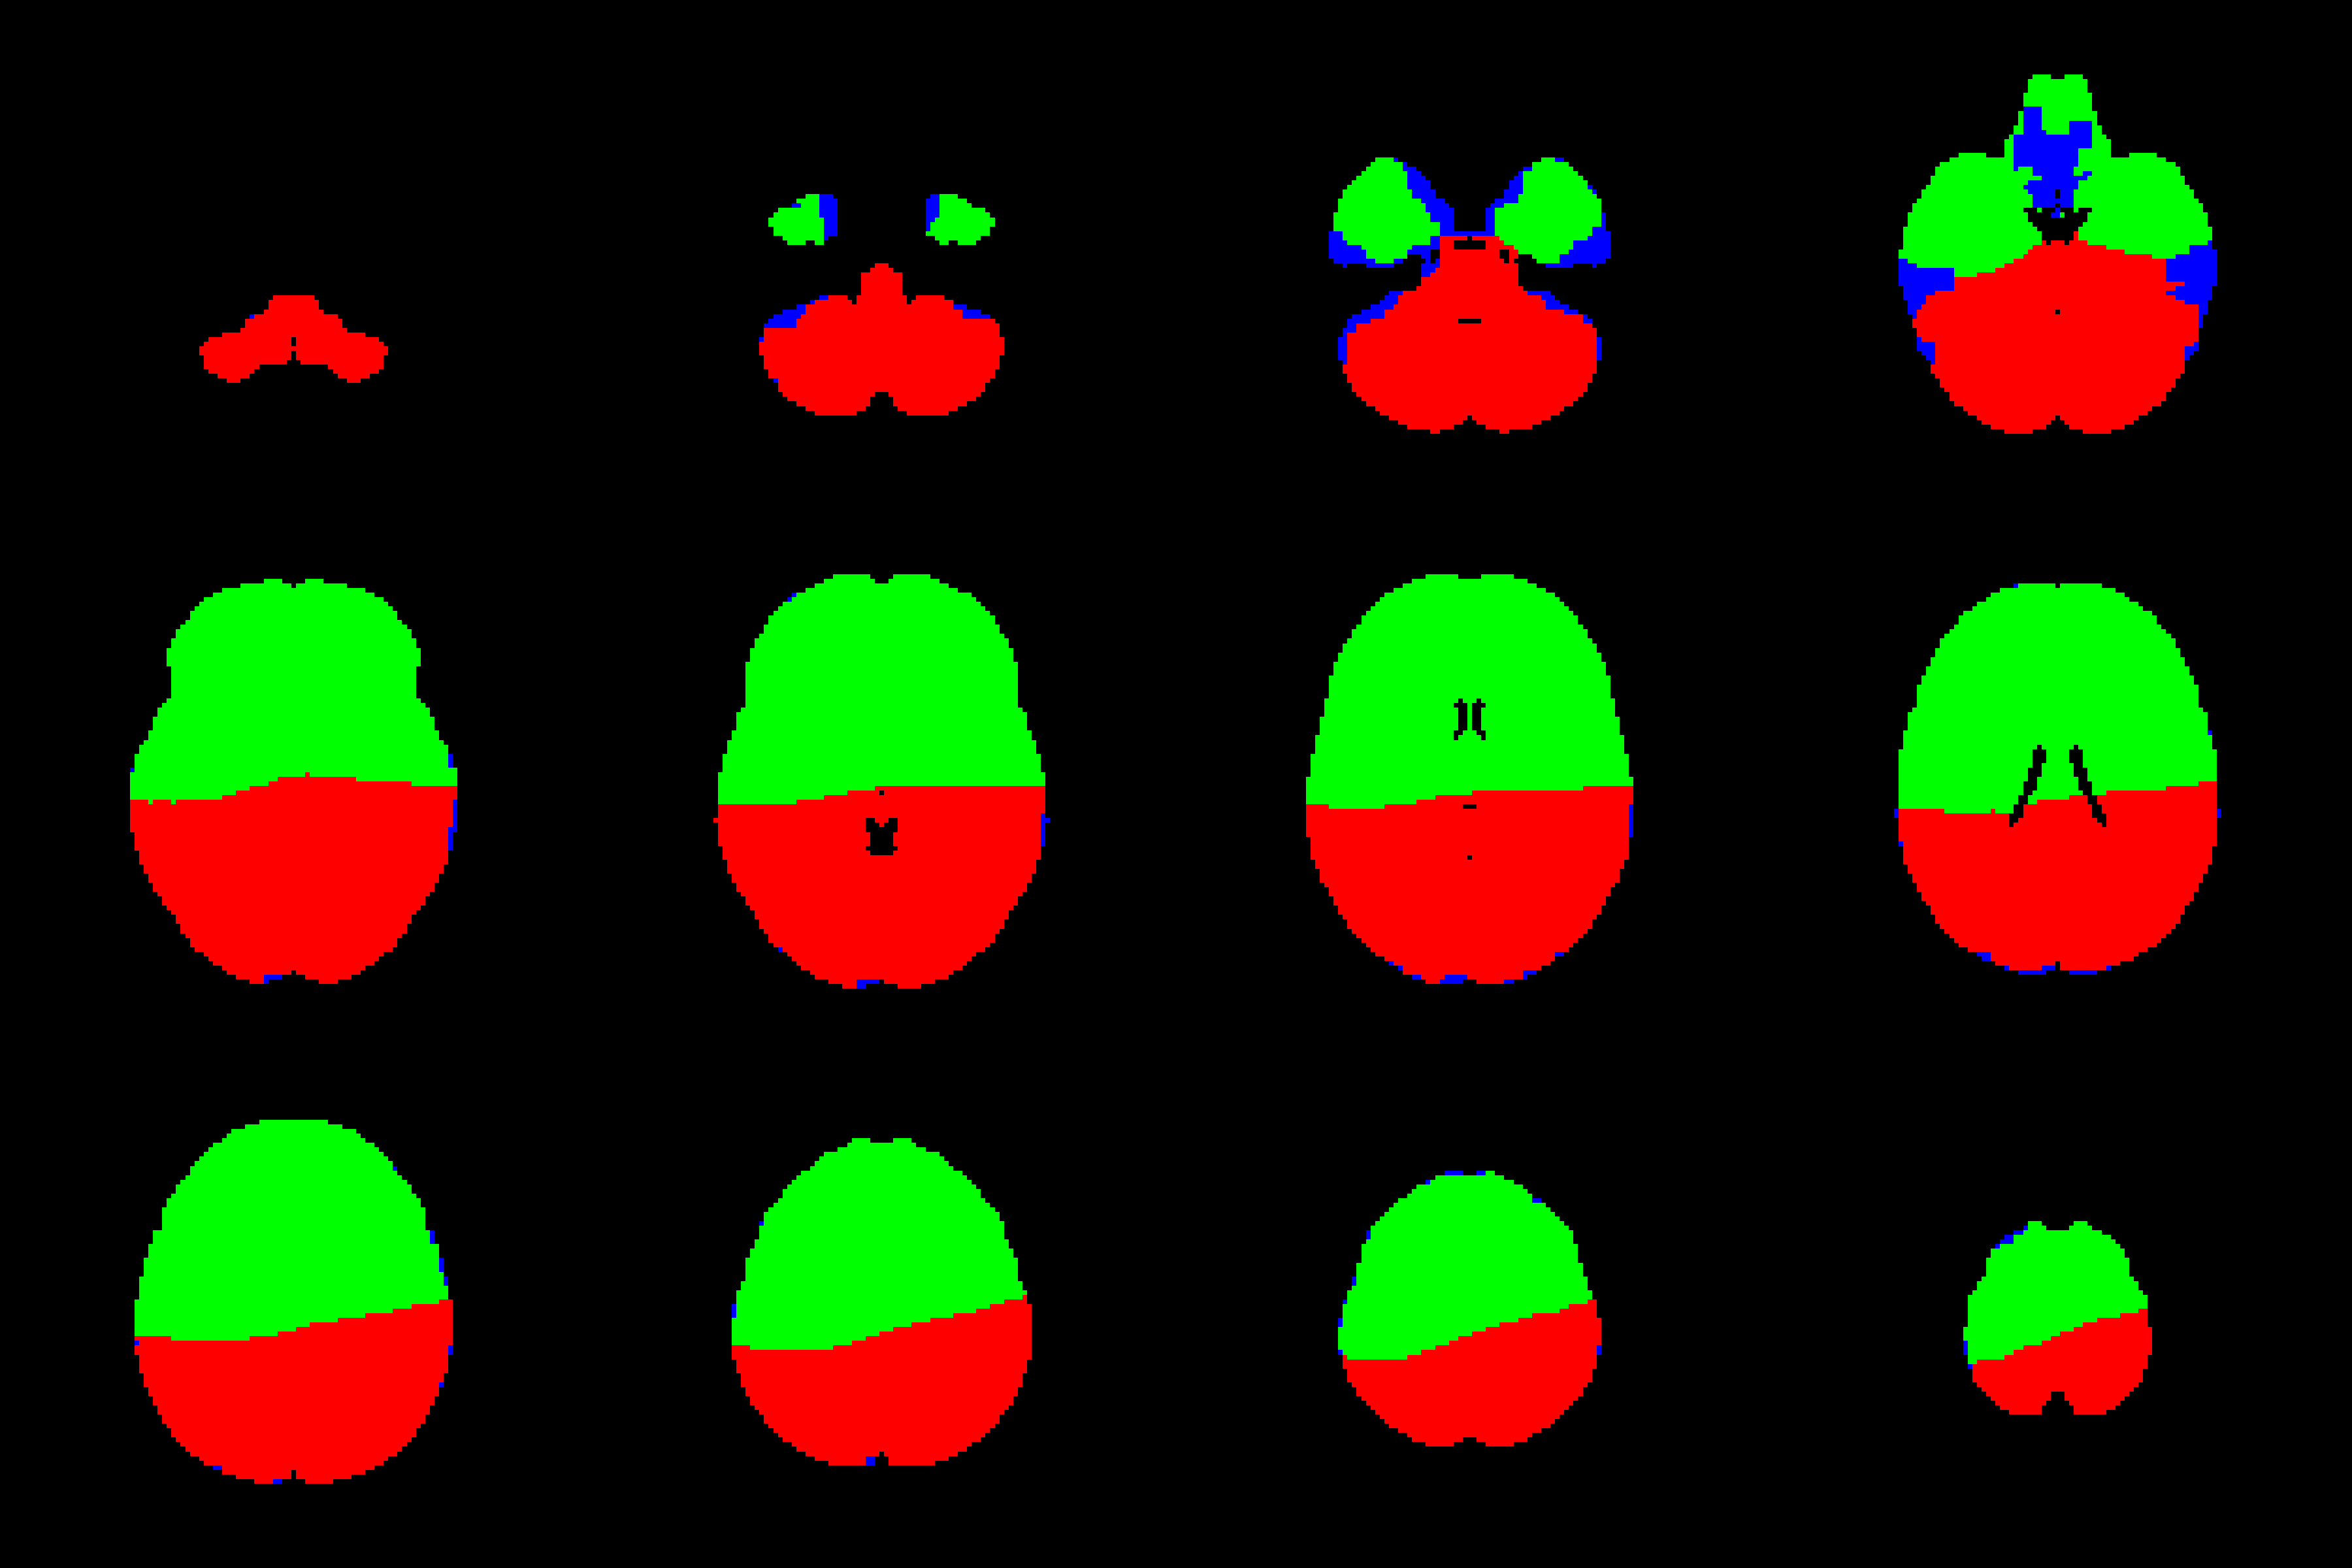
\includegraphics[scale = 0.5]{5_spectral_2_axial.png}

Axial

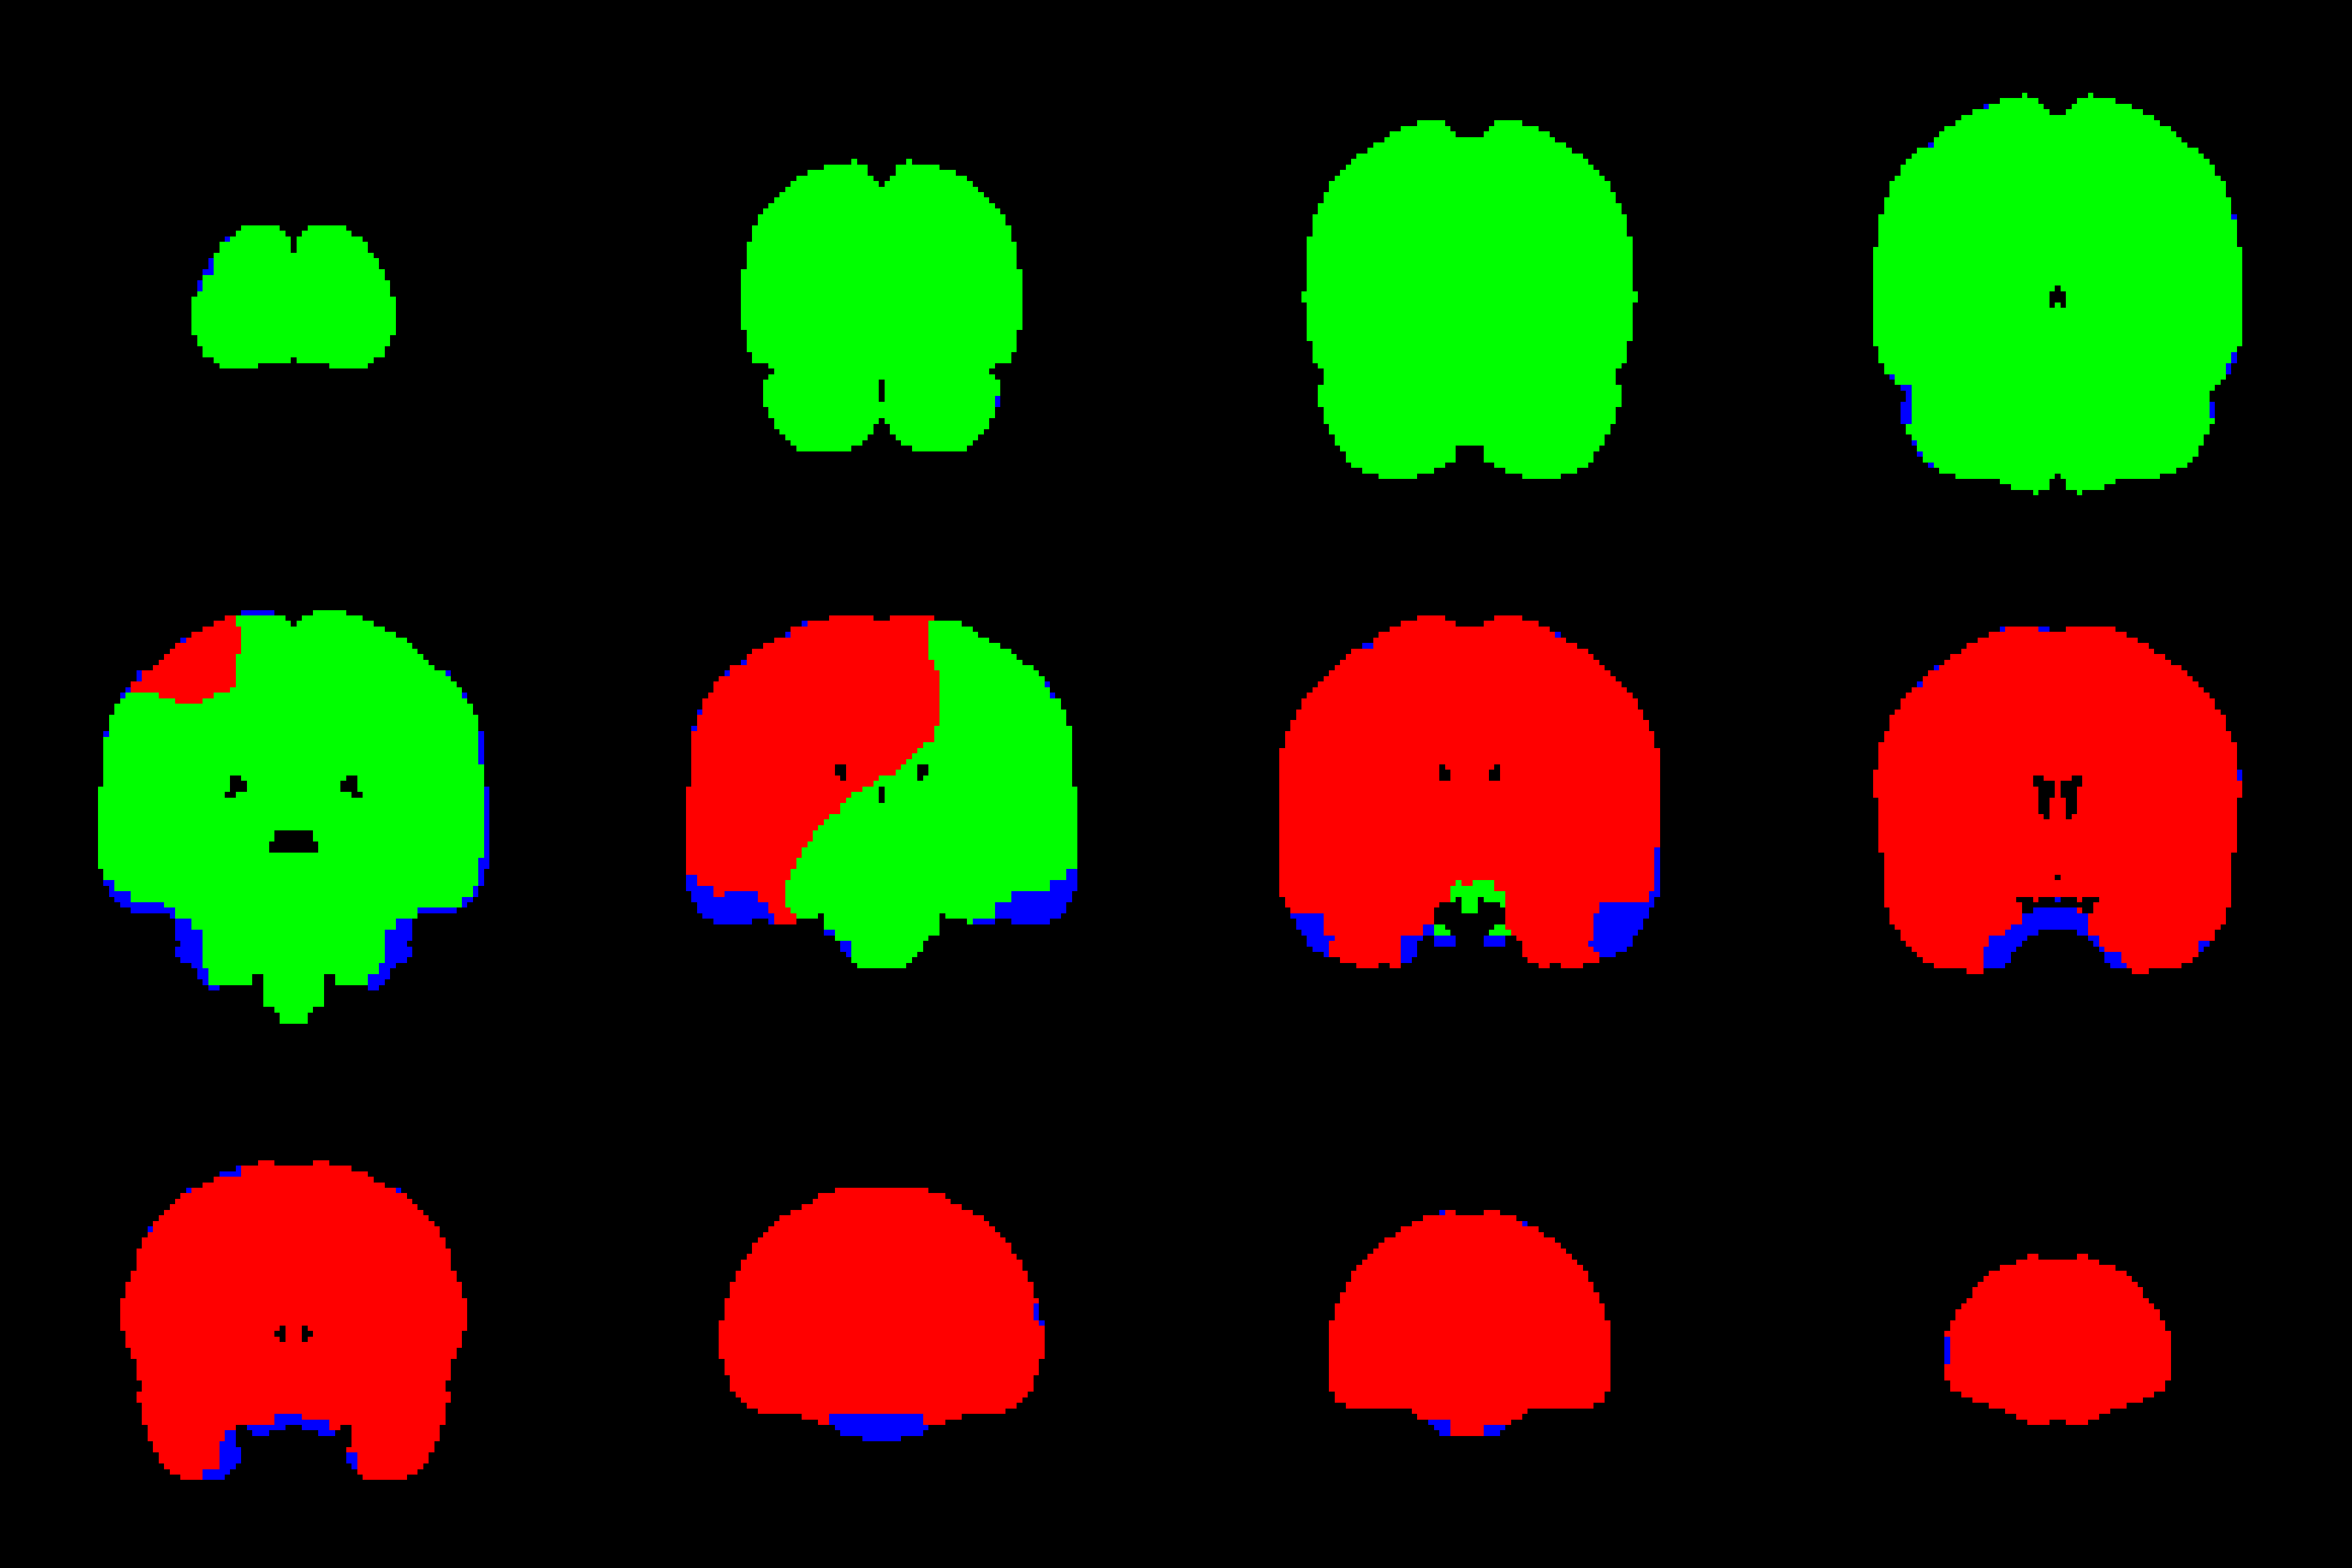
\includegraphics[scale = 0.5]{5_spectral_2_coronal.png}

Coronal

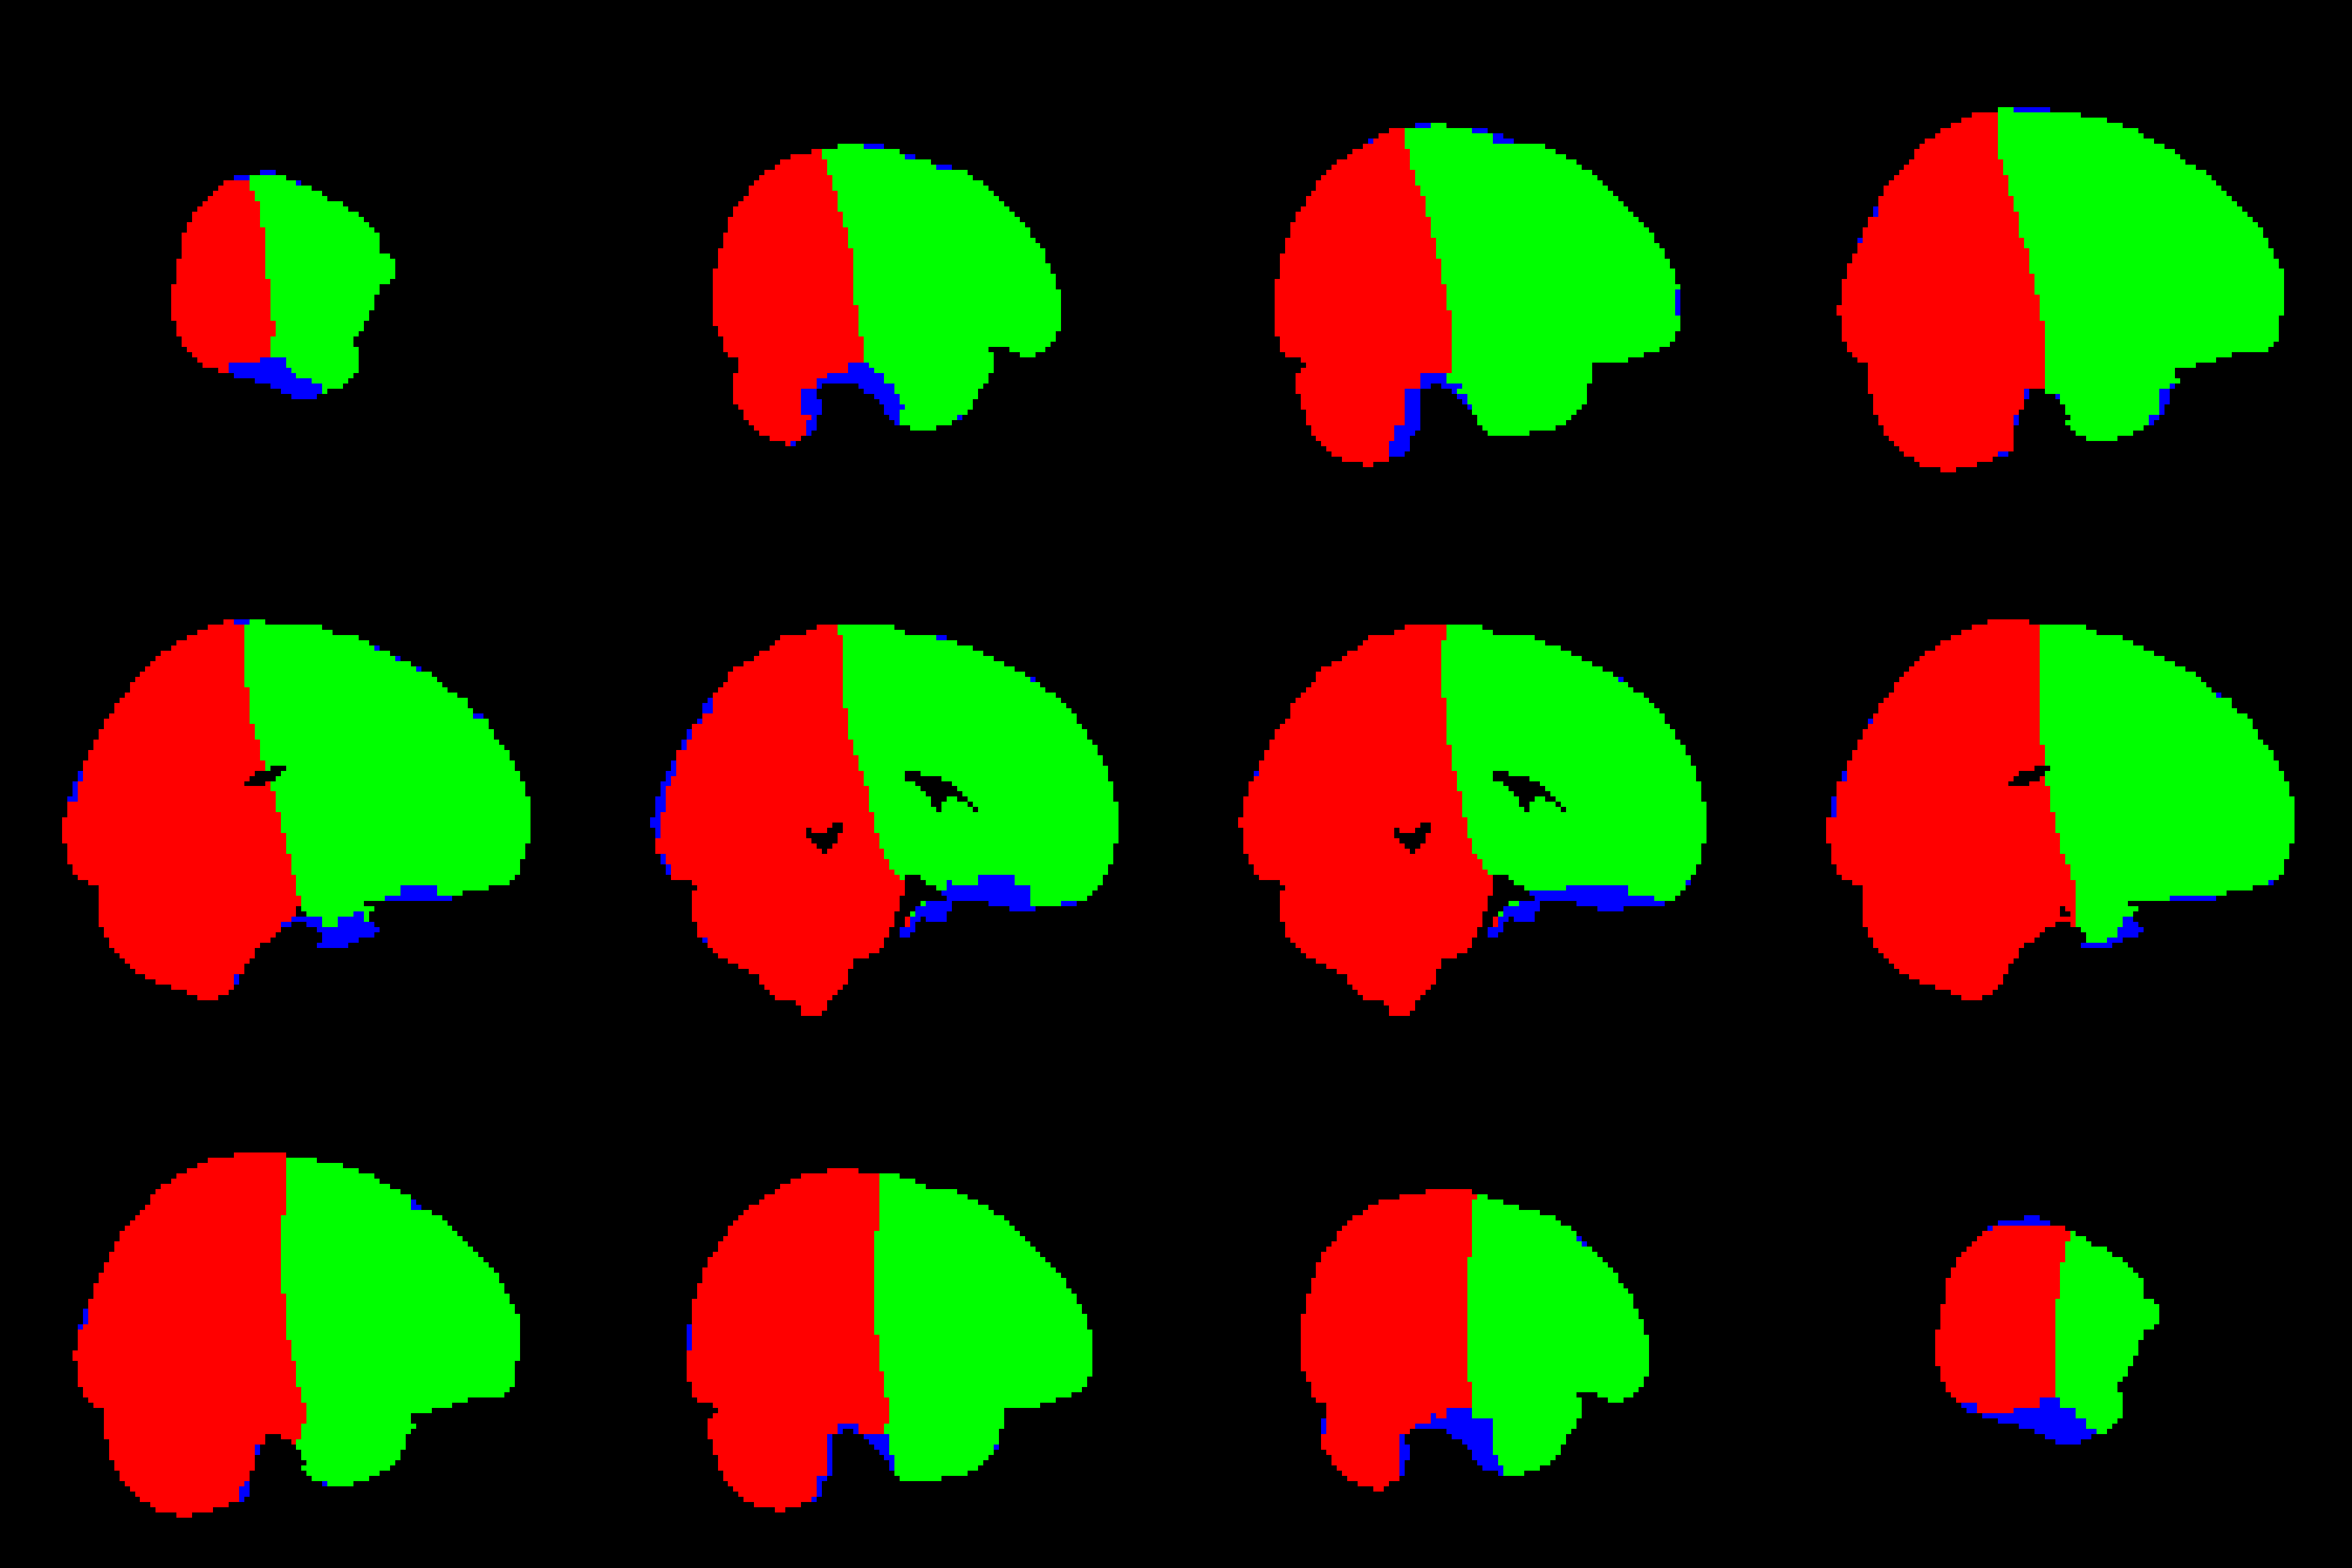
\includegraphics[scale = 0.5]{5_spectral_2_sagittal.png}

Sagittal
\end{center}

One can recursively apply this bipartitioning method to the component
subgraphs to obtain $k$-partitions, but there is a more elegant
approach involving additional eigenvectors that requires the
construction of only one Laplacian matrix, which we shall discuss next.

\section{Spectral k-partitioning}

We'll begin with two definitions to set up the machinery for
partitioning into $k$ components.

\begin{definition}
Assignment matrix. $X \in \{0, 1\}^{n \times k}$ has entries
\[ X_{ih} = \begin{cases}
		1 & \mbox{if vertex } i \in V_h \\
		0 & \mbox{otherwise}
\end{cases} \]
\end{definition}

Let $u_m$ denote a vector of $m$ ones.
An assignment matrix characterizes a valid partition only if it
satisfies $X u_k = u_n$ and $X^T u_n > 0$.
The columns of $X$ are orthogonal.

\begin{definition}
Partition matrix. $P \in \{0, 1\}^{n \times n}$ has entries
\[ P_{ij} = \begin{cases}
		1 & \mbox{if vertices } i \mbox{ and } j
		    \mbox{ are in the same component} \\
		0 & \mbox{otherwise}
\end{cases} \]
\end{definition}

If $P$ and $X$ refer to the same partitioning, then $P = X X^T$.

In the $k$-component case, we define the weight of a partition
$C(P_k)$ as the sum of weights of edges between different components
(between-edges). This is equivalent to the definition below:

\begin{definition}
[Cut weight] For a partition $P_k = (V_1, ..., V_k)$, the cut weight
is defined as
\[ C(P_k) = \sum_{h=1}^k E_h \]
where $E_h$ is the sum of the weights of all edges with one vertex in
$V_h$ and one vertex not in it.
\end{definition}

This is equal to the sum of the weights of all edges in the graph minus
the sum of the weights of all edges connecting vertices in the same
component (within-edges).

In addition, if $D$ is the degree matrix, then
\begin{align*}
\Tr(P D) &= \sum_{i,j = 1}^n P_{ij} D_{ij} \\
         &= \sum_{i=1}^n P_{ii} D_{ii}  \\
         &= \sum_{i=1}^n P_{ii} \sum_{j=1}^n A_{ij} \\
         &= \sum_{i=1}^n \sum_{j=1}^n A_{ij}
\end{align*}
is the sum of the weights of all edges in the graph.
Similarly, $\Tr(P A)$ equals the sum of weights of all within-edges.
It follows that 
\[ C(P_k) = \Tr(X^T L X) \]

The derivation of the spectral relaxation for the multi-partition
problem in [Chan 1994] actually doesn't attempt to minimize $C(P_k)$
directly for reasons to be elaborated below. Rather, it minimizes a
related objective called the ratio-cut cost.

\begin{definition}
[Ratio-cut cost] For a given partition $P_k = (V_1, ..., V_k)$ the
ratio-cut cost $C_R$ is defined
\[ C_R(P_k) = \sum_{h=1}^k \frac{E_h}{|V_h|} \]
where $E_h$ is the sum of the weights of all edges with one vertex in
$V_h$ and one vertex not in it.
\end{definition}

[Chan 1994] defines a new decision variable $R$, of the same form as
$X$ but with columns rescaled so that the column sum is $\sqrt{|V_h|}$
for each component $V_h$.

\begin{definition}
[Ratioed Assignment Matrix] $R \in \R^{n \times k}$ has entries
\[ R_{ih} = \begin{cases}
		\frac{1}{\sqrt{|V_h|}} & \mbox{if vertex } i \in V_h \\
		0 & \mbox{otherwise}
\end{cases} \]
\end{definition}

The ratioed assignment matrix relates to the ratio-cut cost in the same
way the assignment matrix relates to cut weight; namely, if $R$
characterizes a partition $P_k$ then
\[ C_R(P_k) = \Tr(R^T L R) \]
$R$ has the additional useful property that $R^T R = I$. This property
leads to a closed form optimal solution to

\begin{equation} \label{spectral_k-partition}
\begin{aligned}
\min_{R \in \R^{n \times k}} &\;& \Tr(R^T L R) \\
\text{s.t.}                  &\;& R^T R = I    \\
\end{aligned}
\end{equation}

[Fan 1949] proved that an optimal solution $\hat{R}$ to the above
consists of $k$ orthonormal eigenvectors corresponding to the $k$
smallest eigenvalues of $L$. Analogously to $P = X X^T$,
$\hat{R}$ can be thought of as $n$ $k$-dimensional points where the
dot products of the $i$th and $j$th rows measure the affinity of
vertices $i$ and $j$ to be in the same component.

As [Chan 1994] pointed out, recovery of the discrete assignment matrix
$X$ from the continuous assignment matrix $\hat{R}$ would be more
accurate if $\hat{R}$ were un-ratioed (i.e. if each row of $R$ had the
same length), since the ratioed assignment matrix $R$ has the
problematic property that for any $i,j$ in the same component, the dot product $R_i^T R_j$ depends on the size of that component.
The un-ratioed version of $\hat{R}$ be recovered by dividing each row
by its Euclidean norm. The result, $\hat{X}$, can be thought of as $n$
points in $\R^k$ embedded on the surface of the unit hypersphere.

Obtaining the partition assignment matrix $X$, from this spherical
embedding is a clustering problem. We used k-means with cosine
similarity $s(x,y) = x^T y$ for this purpose. For each cluster $h$
and its associated points matrix $H \in \R^{m \times k}$, the
location of the cluster centroid $c_h$ in the next iteration satisfies
$ \sum_{i=1}^m H_i = \lambda c_h $ for some positive scalar $\lambda$
such that $ \| c_h \| = 1$.

To summarize, [Chan 1994] introduced a spectral relaxation of the graph
$k$-partitioning to minimize the ratio cut. From the Laplacian matrix's
smallest $k$ eigenvectors we obtain a continuous approximation $\hat{R}$
to the optimal ratioed assignment matrix $R$. The rows of $\hat{R}$ are
standardized to length 1 to get the continuous approximation $\hat{X}$
to optimal (unratioed) assignment matrix $X$. Our modification of
this method uses k-means clustering with cosine similarity to recover
the component assignments from $\hat{X}$.

\section{Comparison of Parcellations using Recursive Bipartitioning
and k-Partitioning}


\section{Equivalence of Spectral K-Partitioning and Adjacency Matrix
Embedding}


%#######################################################################
